
\clearpage
\appendix

\section*{Appendix}
\section{Metric: \texttt{Dependency}}
\label{sec:app:metric}
\begin{figure}[!htbp] % !t, !htbp
    \centering
    \scalebox{1}{
    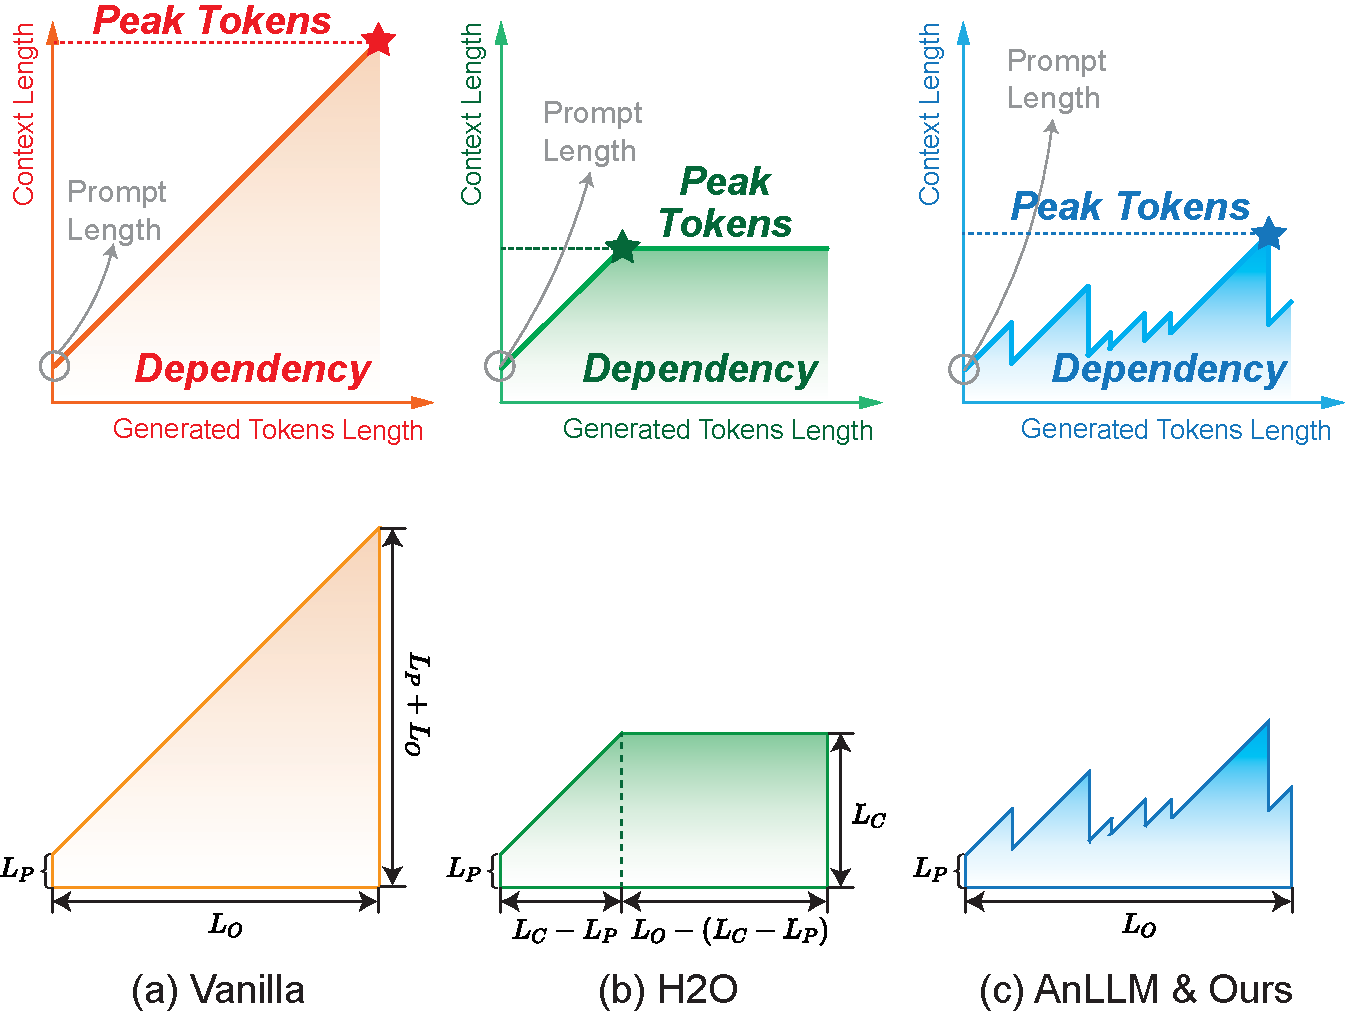
\includegraphics[width=1.0\linewidth]{figures/metric-cal-v1.pdf} 
    }
    % \vspace{-1mm}
    \caption{Illustration of the metric Dependency.}
    \label{fig:app:metric}
    % \vspace{-3mm}
\end{figure} 
\subsection{Motivation}
\ours~and AnLLM~\citep{acl24_anllm} are dynamic compression methods, meaning the number of compressions and the compression ratio are determined by the LLM itself rather than being predefined hyperparameters. 
In contrast, H2O~\citep{nips23_h2o} and SepLLM~\citep{arxiv24_sepllm} allow users to set hyperparameters to control the maximum number of tokens retained during inference. 
This fundamental difference makes it challenging to directly and fairly compare dynamic compression methods like \ours~and AnLLM with KV cache compression approaches like H2O and SepLLM.  

Traditionally, KV cache compression methods are compared by setting the same maximum peak token count, but this metric becomes inadequate in our context. 
As illustrated in Figure~\ref{fig:app:metric}, which shows the relationship between generated tokens and context length for Vanilla, H2O, and \ours, 
\ours~occasionally exceeds H2O in peak token count. 
However, this metric is misleading because \ours's peak memory usage occurs only momentarily, while H2O maintains a consistently high token count over time.  

Moreover, previous KV cache compression methods often compress prompt parts only and assume a fixed prompt length, allowing compression ratios to be predefined. 
In our setting, however, the output is also needed to be compressed.
The output token count is unknown, making it impossible to preset a global compression ratio. 
Consequently, relying solely on maximum peak token count as a comparison metric is insufficient.  

To address these challenges, we propose a new metric called \textit{Dependency}, which quantifies the total amount of information dependencies during the generation process. 
This metric enables fair comparisons between dynamic compression methods and traditional KV cache compression approaches by ensuring evaluations are conducted under similar effective compression ratios.  
\subsection{Definition}
We introduce the \textbf{Dependency} (abbr., Dep) metric, defined as the sum of dependencies of each generated token on previous tokens during the generation of an output. 
Geometrically, it represents the area under the curve in Figure~\ref{fig:app:metric}. 
Dependency can be calculated either from its definition or through its geometric interpretation. 
Here, we focus on the geometric approach. 
Let the initial prompt length be \( L_P \), the model's output length be \( L_O \), and the maximum context length set by KV cache compression methods be \( L_C \).  

\textbf{Dependency for Vanilla.}
The area under Vanilla's curve forms a right trapezoid, calculated as:  
\[
\begin{aligned}
\texttt{Dependency} &= \frac{(L_P + L_P + L_O) \times L_O}{2} \\
&= \frac{{L_O}^2}{2} + L_P \times L_O
\end{aligned}
\]

\textbf{Dependency for H2O.}
The area under H2O's curve consists of a trapezoid (left part in Figure~\ref{fig:app:metric}(b)) and a rectangle (right part in Figure~\ref{fig:app:metric}(b)):  
\[
\begin{aligned}
S_\texttt{Trapezoid} &= \frac{(L_P + L_C) \times (L_C - L_P)}{2} \\
S_\texttt{rectangle} &= L_C \times (L_O - L_C + L_P) \\
\texttt{Dependency} &= S_\texttt{Trapezoid} + S_\texttt{rectangle} \\
&= \frac{2L_PL_C + 2L_OL_C - {L_P}^2 - {L_C}^2}{2}
\end{aligned}
\]

\textbf{Dependency for \ours~and AnLLM.}
For \ours~and AnLLM, Dependency does not have a closed-form solution and must be computed iteratively based on its definition. 

\subsection{Application}
\textbf{Value of Dependency.}
A higher Dependency value indicates that more tokens need to be considered during generation, reflecting greater information usage.
Conversely, a lower Dependency value suggests a higher effective compression ratio.  

\textbf{Dependency Ratio.}
By dividing the Dependency of an accelerated method by that of Vanilla, we obtain the compression ratio relative to Vanilla. For example, in Table~\ref{table:exp_main}'s ``Avg.'' column, Vanilla's Dependency is 16.6M, H2O's is 4.4M, and \ours's is 3.7M. 
Thus, H2O achieves a compression ratio of \( \frac{16.6}{4.4} \approx 3.8 \), while \ours~achieves \( \frac{16.6}{3.7} \approx 4.5 \).  

This metric provides a unified framework for evaluating both dynamic and static compression methods, ensuring fair and meaningful comparisons.

% \section{Inference Pseudocode}


\begin{figure}[!htbp] % !t, !htbp
    \centering
    \scalebox{1}{
    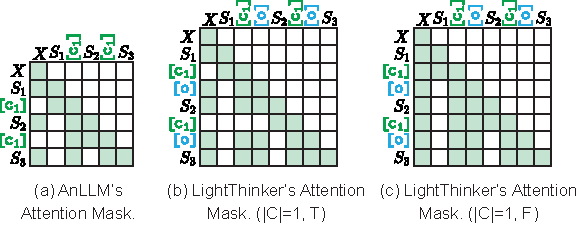
\includegraphics[width=1.0\linewidth]{figures/attention_mode-v1.pdf} 
    }
    % \vspace{-1mm}
    \caption{Illustration of Attention Mask in Table~\ref{table:exp:ablation:attention}.}
    \label{fig:app:attention_mode}
    % \vspace{-3mm}
\end{figure} 
\section{Mathematical Description of Compression}
\label{sec:app:compress}
In this section, we provide a detailed formulation of the compression operation introduced in Section~\ref{sec:method:method}.

\paragraph{Notation.} 
During compression, the context can be divided into three segments: 
1. The sequence that remains in the context without being compressed, denoted as $Pre := \{X, \{C^{(1)}, \texttt{[o]}^{(1)}\dots,C^{(i-1)},\texttt{[o]}^{i-1}\}\}$, with the number of tokens represented by $N$; 
2. The thought sequence to be compressed, defined as $Tho:=S_i$, with the number of tokens denoted by $T$; 
3. The sequence storing the compressed content, $C:=C^{(i)}$, with its length represented by $|C|$.

\paragraph{Compression Operation.} 
Here, we describe the compression operation at a specific layer, focusing on the information passed to the sequence $C$. 
According to the definition of self-attention~\citep{nips17_transformer}, the attention matrix for the sequence $C$ with respect to other content is calculated as:
\[
A=\text{Softmax}(\text{mask}(\frac{Q^{C}[K^{Pre}:K^{Tho}:K^{C}]^{\top}}{\sqrt{d}}))
\]
where $[:]$ denotes the concatenation operation, $\text{mask}(\cdot)$ represents the attention mask corresponding to the ``Thought-based Attention Mask Construction'' in Section~\ref{sec:method:method}, 
$K^{Pre}, V^{Pre}\in \mathbb{R}^{N\times d}$, 
$K^{Tho}, V^{Tho}\in \mathbb{R}^{T\times d}$, 
$K^{C},V^{C}\in \mathbb{R}^{|C|\times d}$, $Q^{C}\in \mathbb{R}^{|C|\times d}$, 
and $d$ is the hidden dimension. The matrix $A\in \mathbb{R}^{|C|\times (N+T+|C|)}$ describes the attention of sequence $C$ to other content. 
The \textit{values} of the other sequences are then weighted and summed according to the attention matrix:
\[
H=A\times [V^{Pre}:V^{Tho}:{V^C}]
\]
where $[V^{Pre}:V^{Tho}:V^{C}]\in \mathbb{R}^{(N+T+|C|)\times d}$,
and thus $H\in \mathbb{R}^{|C|\times d}$. 
At this point, the information from the current $Tho$ is preserved in $H$. 
Through training, the model learns to selectively retain useful information from $Tho$ in $H$. 
$H$ is then stored in the KV Cache after passing through an MLP and the next layer's projection.


\section{Experiment}
% The code and data will be released at \url{https://github.com/zjunlp/LightThinker}.
\label{sec:app:exp}
\subsection{Training Data}
\label{sec:app:exp:train_data_case}
Examples of training samples are shown in Figure~\ref{prompt:case:train}.

\subsection{Baseline Details}
\label{sec:app:exp:baseline_details}
\textbf{H2O}~\citep{nips23_h2o} is a training-free acceleration method that greedily retains tokens with the highest cumulative attention values from historical tokens. 
It includes two hyper-parameters: the maximum number of tokens and the current window size (i.e., \texttt{local\_size}). 
The maximum number of tokens for each task is listed in the ``Peak'' column of Table~\ref{table:exp_main}, and the \texttt{local\_size} is set to half of the maximum number of tokens. 
The experimental code is implemented based on \url{https://github.com/meta-llama/llama-cookbook}.

\textbf{SepLLM}~\citep{arxiv24_sepllm} is another training-free acceleration method that considers tokens at punctuation positions as more important. 
It includes four parameters: the maximum number of tokens is set to 1024, \texttt{local\_size} is set to 256, \texttt{sep\_cache\_size} is set to 64, and \texttt{init\_cache\_size} is set to 384. 
We also tried another set of parameters (\texttt{init\_cache\_size}=4, \texttt{sep\_cache\_size}=64, \texttt{local\_size}=720, maximum number of tokens=1024), but found that the first set of parameters performed slightly better.

\textbf{AnLLM}~\citep{acl24_anllm} is a training-based method that shares a similar overall approach with \ours~but accelerates by saving historical content in anchor tokens. 
The specific differences between the two are detailed in Section~\ref{sec:app:discussion}.

\subsection{Training Details}
\label{sec:app:exp:training_details}
Both \textbf{Vanilla} and \textbf{AnLLM} are trained on the B17K~\citep{bespoke_stratos_train_dataset} dataset using the R1-Distill~\citep{arxiv25_deepseek_r1} model for 5 epochs, while \ours~is trained for 6 epochs. 
The maximum length is set to 4096, and a cosine warmup strategy is adopted with a \texttt{warmup\_ratio} of 0.05. 
Experiments are conducted on 4 A800 GPUs with DeepSpeed ZeRo3 offload enabled. 
The batch size per GPU is set to 5, and the gradient accumulation step is set to 4, resulting in a global batch size of 80. 
The learning rate for Vanilla is set to 1e-5, while for AnLLM and \ours, it is set to 2e-5.

\subsection{Evaluation Details}
\label{sec:app:exp:evaluation_details}
For the CoT in Table~\ref{table:exp_main}, the prompts used are shown in Figure~\ref{prompt:system:base} and Figure~\ref{prompt:task:base}. 
For the R1-Distill model, no system prompt is used, and the task-specific prompts are shown in Figure~\ref{prompt:task:r1}. 
Vanilla, H2O, SepLLM, AnLLM, and \ours~share the same set of prompts, with the system prompt shown in Figure~\ref{prompt:system:vanilla} and downstream task prompts shown in Figure~\ref{prompt:task:r1}. 
The options for MMLU~\citep{iclr21_mmlu} and GPQA~\citep{colm24_gpqa} multiple-choice questions are randomized.

\subsection{Additional Results}
\label{sec:app:exp:additional_results}
Figure~\ref{fig:app:token} compares the number of tokens generated by two models across different datasets. 
Figure~\ref{fig:app:frequency} shows the distribution of compressed lengths for LightThinker on two models and four datasets. Figure~\ref{fig:app:attention_mode} illustrates the attention masks for the baselines in Table~\ref{table:exp:ablation:attention}.
Figure~\ref{prompt:case} shows a complete case in Figure~\ref{fig:exp:case}.

\begin{figure*}[!htbp] % !t, !htbp
    \centering
    \scalebox{0.8}{
    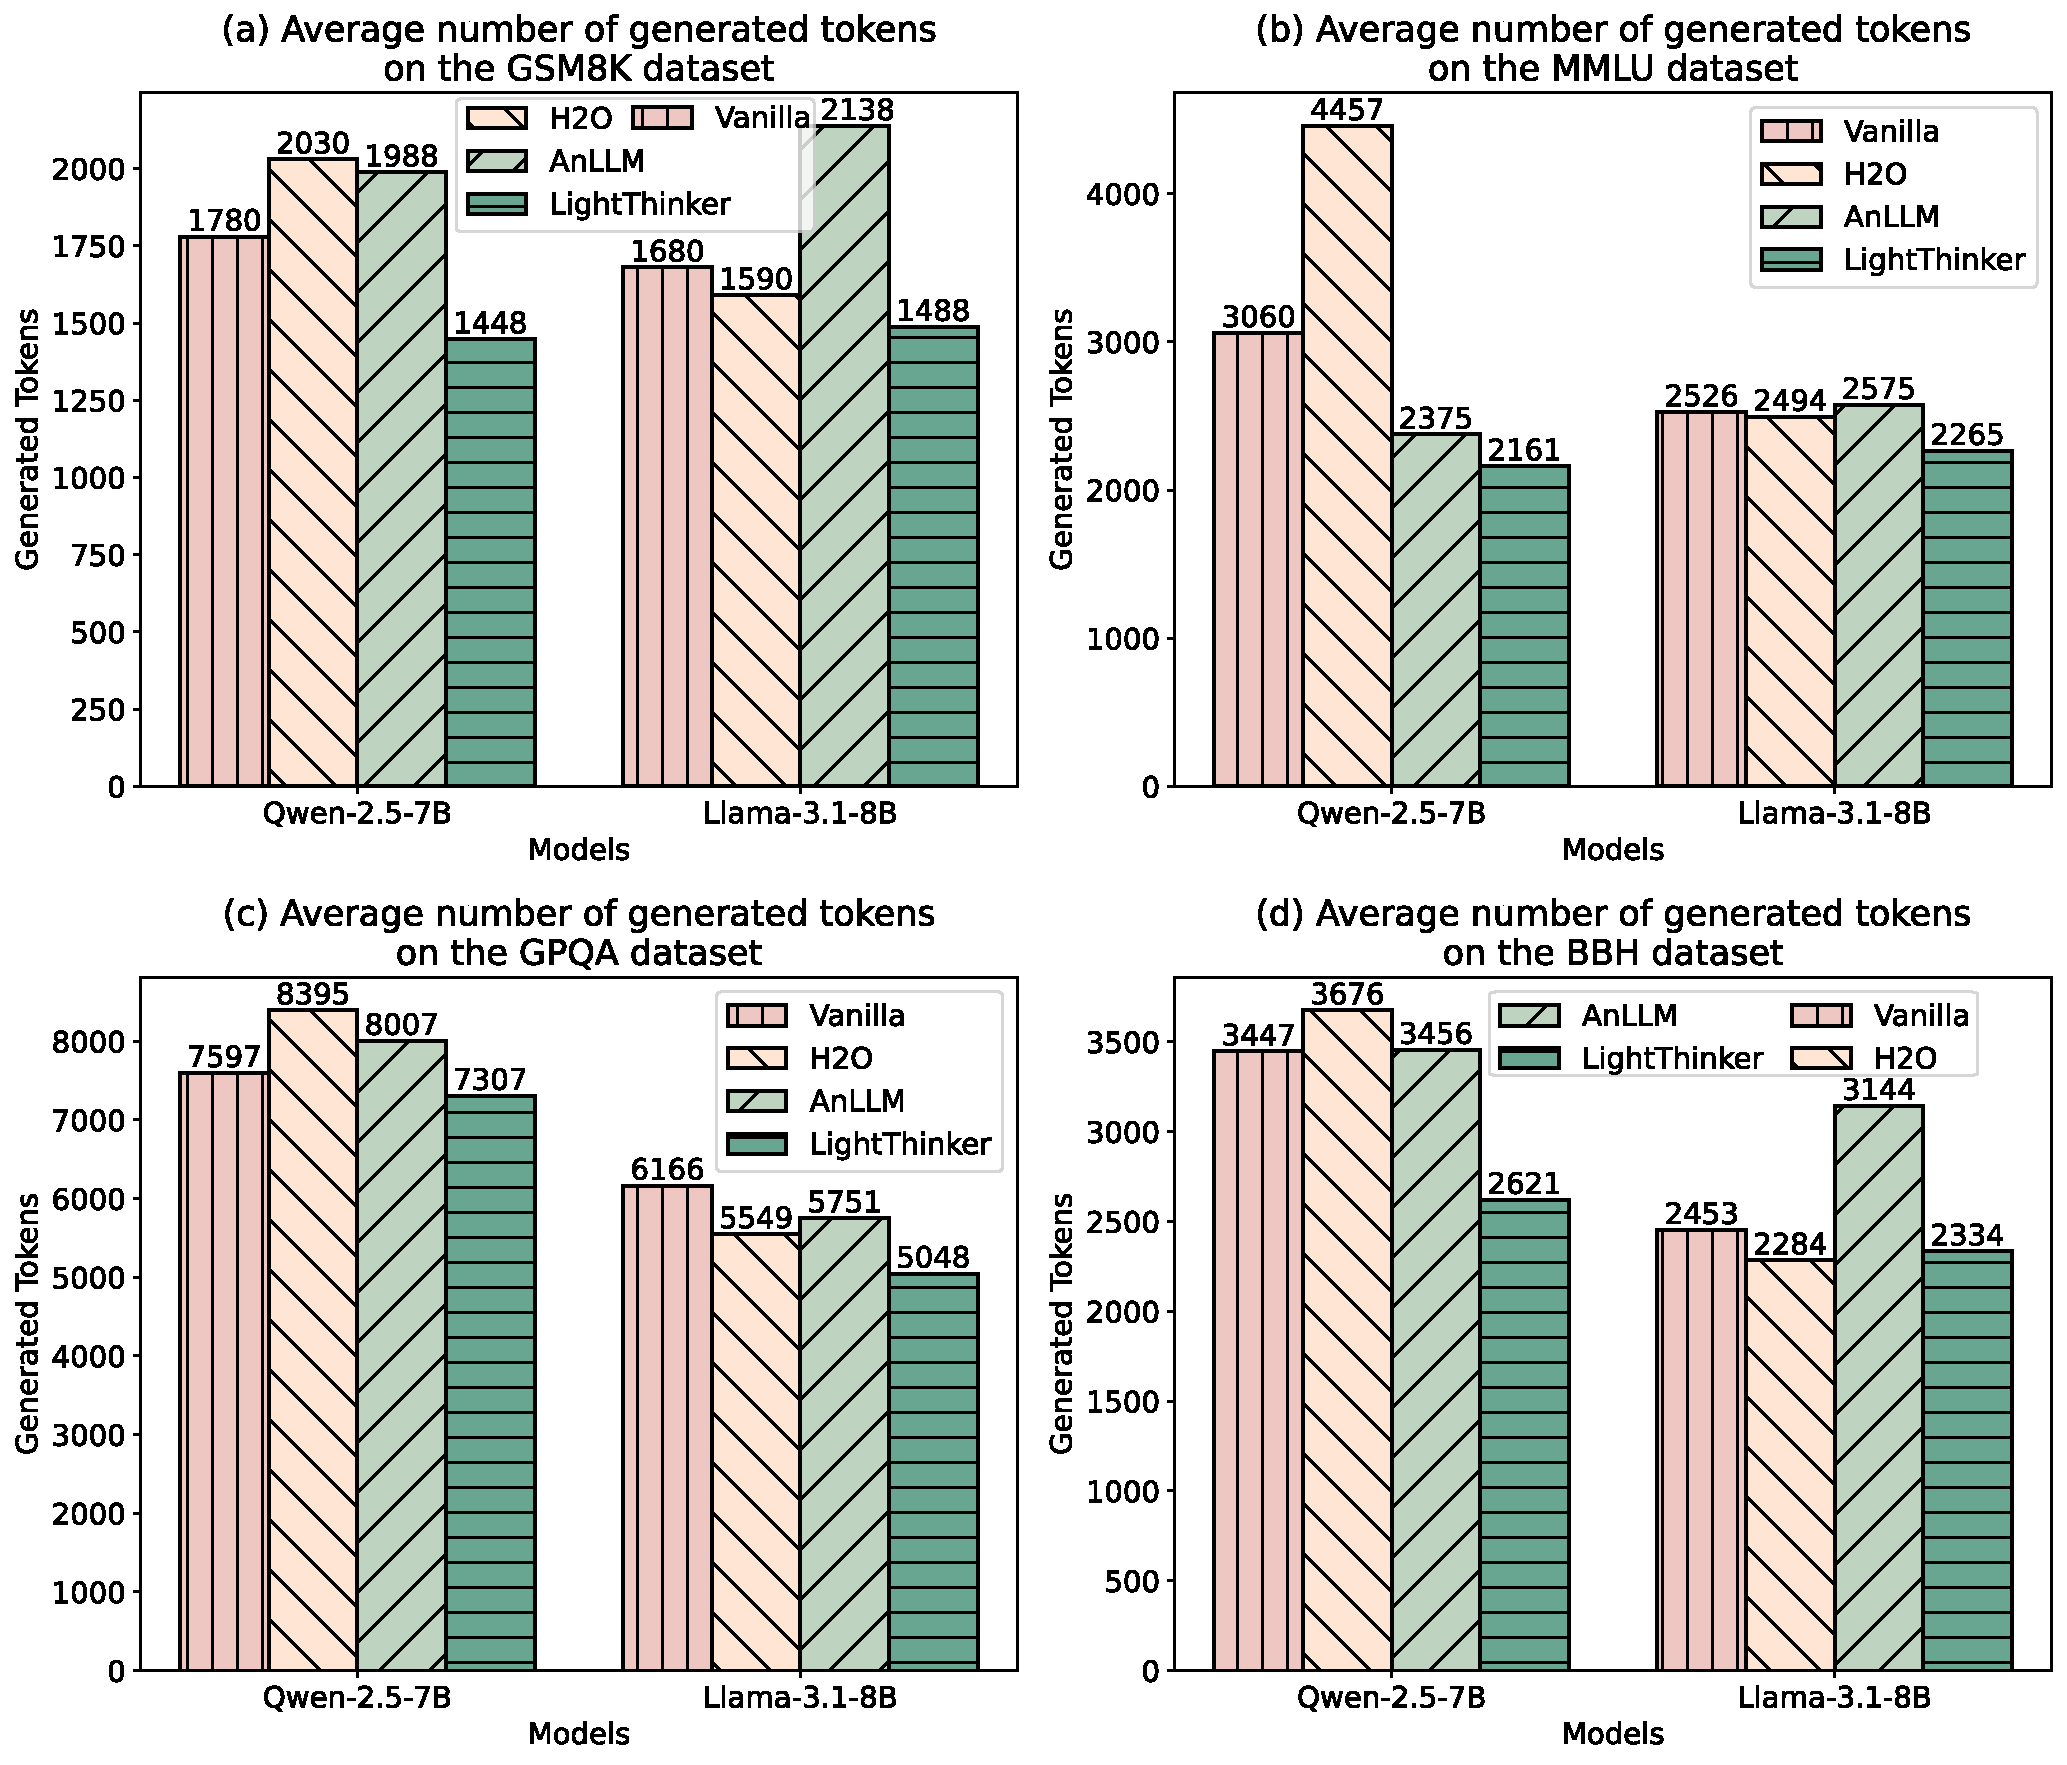
\includegraphics[width=1.0\linewidth]{figures/token_split-v2.pdf} 
    }
    % \vspace{-1mm}
    \caption{Average number of generated tokens.}
    \label{fig:app:token}
    % \vspace{-3mm}
\end{figure*} 

\section{Related Work}
\label{sec:app:related_work}

Current research on accelerating the inference process of large language models (LLMs) primarily focuses on three categories of methods: \textit{Quantizing Model}, \textit{Generating Fewer Tokens}, and \textit{Reducing KV Cache}. 
Quantizing Model includes both parameter quantization~\cite{mlsys24_awq,nips22_8bit} and KV Cache quantization~\citep{icml24_kivi,nips24_kvquant}, while this section will concentrate on the latter two categories. 
It is important to note that generating long texts and understanding long texts represent distinct application scenarios; 
therefore, acceleration methods specifically targeting the long-text generation phase (e.g., pre-filling stage acceleration techniques such as AutoCompressor~\citep{emnlp23_autocompressors}, ICAE~\citep{iclr24_icae}, LLMLingua~\citep{emnlp23_llmlingua}, Activation Beacon~\citep{iclr25_activation_beacon}, SnapKV~\citep{nips24_snapkv}, and PyramidKV~\citep{arxiv24_pyramidkv}) are not discussed here. 
Below is a detailed overview of the last two categories.

\textbf{Generating Fewer Tokens.}
This category can be further divided into three strategies based on the number and type of tokens used during inference.
1) \textit{Discrete Token Reduction}. 
Techniques such as prompt engineering~\citep{arxiv24_tale,arxiv24_break_the_chain,arxiv24_concise_thoughts}, instruction fine-tuning~\citep{nips24_skip_steps,arxiv24_c3ot}, or reinforcement learning~\citep{arxiv25_related_work_rl1,arxiv25_o1_pruner} are used to guide LLMs to use fewer discrete tokens during inference.
For example, TALE~\citep{arxiv24_tale} prompts LLMs to complete tasks under a predefined token budget. 
\citeauthor{arxiv25_related_work_rl1} construct specific datasets and employ reinforcement learning reward mechanisms to encourage models to generate concise and accurate outputs, thereby reducing token usage.
2) \textit{Continuous Token Replacement}.
These methods~\citep{arxiv24_coconut,arxiv24_ccot} explore using continuous-space tokens instead of traditional discrete vocabulary tokens. 
A representative example is CoConut~\citep{arxiv24_coconut}, which leverages Curriculum Learning to train LLMs to perform inference with continuous tokens.
3)\textit{No Token Usage}.
By internalizing the inference process between model layers, the final answer is generated directly during inference without intermediate tokens~\citep{arxiv24_icot,arxiv23_kd_cot}.
These three strategies are implemented after model training and do not require additional intervention during inference. 
Technically, the acceleration effect of these methods increases sequentially, but at the cost of a gradual decline in the generalization performance of LLMs. 
Additionally, the first strategy does not significantly reduce GPU memory usage.

\textbf{Reducing KV Cache.}
This category can be divided into two types of strategies: pruning-based KV Cache selection in discrete space and merging-based KV Cache compression in continuous space.
1) \textit{Pruning-Based Strategies}.
Specific eviction policies~\citep{nips23_h2o, iclr24_streamingllm,arxiv24_sepllm,arxiv24_scope} are designed to retain important tokens during inference.
For example, StreamingLLM~\citep{iclr24_streamingllm} considers the initial sink tokens and the most recent tokens as important.
H2O~\citep{nips23_h2o} focuses on tokens with high historical attention scores.
SepLLM~\citep{arxiv24_sepllm} emphasizes tokens corresponding to punctuation marks.
2) \textit{Merging-Based Strategies}.
Anchor tokens are introduced, and LLMs are trained to compress historically important information into these tokens, thereby achieving KV Cache merging~\citep{acl24_anllm}.
Both strategies require intervention during inference. 
The key difference is that the first strategy is training-free but applies the eviction policy for every generated token, while the second strategy is a training-based method and allows the LLM to decide when to apply the eviction policy.


\section{Discussions}
\label{sec:app:discussion}
\subsection{Difference between LightThinker and AnLLM}
AnLLM~\citep{acl24_anllm} is a work from 2023, at which time the concept of long-cot~\citep{arixv24_o1,arxiv25_deepseek_r1} did not exist. 
AnLLM itself focuses more on prompt compression rather than output compression. 
Additionally, our method decouples compression and generation, allowing for scaling the number of cache tokens—something AnLLM cannot do. 
Therefore, our work is only related to AnLLM in that both use sparse attention~\citep{nips23_h2o,nips24_snapkv} to speed up processes, but they are not similar works.

AnLLM is a method related to ours.
% , capable of compressing the thought during inference
In Figure~\ref{fig:comp}, we compare the differences in Attention Mask between \ours~and AnLLM:
1) \textit{Decoupling Generation and Compression.}
In AnLLM, the $\texttt{[c}_\texttt{i}\texttt{]}$ token is tasked with both compressing historical information and generating subsequent content, as shown by the blue and pink arrows in Fig.~\ref{fig:comp}. 
This design tightly couples generation and compression. 
In contrast, \ours~decouples these tasks: the $\texttt{[c}_\texttt{i}\texttt{]}$ token solely compresses historical information, while the $\texttt{[o]}$ token performs reasoning based on the compressed content.
2) \textit{Context Visibility during Compression.}
AnLLM can only access the current thought during compression.
% For instance, when compressing $S_2$, only $S_2$ is visible, while the question $X$ and historical compressed content remain inaccessible.
\ours, however, allows access to $X$, historical compressed content, and the current thought during compression, thereby enhancing contextual understanding.
Ablation experiments in Section~\ref{ablation} demonstrate that these designs significantly improve performance.
\begin{figure}[!htbp] % !t, !htbp
    \centering
    \scalebox{1}{
    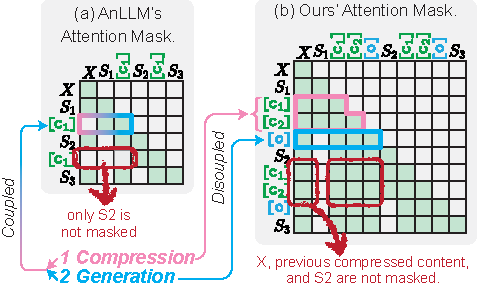
\includegraphics[width=1.0\linewidth]{figures/comp-anllm-v4.pdf} 
    }
    % \vspace{-1mm}
    \caption{
    Contrast of AnLLM and ours.
    Two differences are marked: one with a red box, and the other with blue and pink arrows.
    }
    \label{fig:comp}
    % \vspace{-3mm}
\end{figure} 



\subsection{Viewing \ours~from Other Perspectives}
In previous sections, we design \ours~from a compression perspective. 
Here, we further discuss it from the perspectives of \textit{Memory} and \textit{KV Cache Compression}, where KV Cache can be viewed as a form of LLM work memory.

In Memory perspective, \ours's workflow can be summarized as follows: it first performs autoregressive reasoning, then stores key information from the reasoning process as memory (memory), and continues reasoning based on the memorized content. 
Thus, the information in the cache tokens acts as a compact memory, though it is only effective for the current LLM and lacks transferability.

In KV Cache Compression perspective,
unlike methods such as H2O~\citep{nips23_h2o}, which rely on manually designed eviction policy to select important tokens, \ours~merges previous tokens in a continuous space, \textit{ceating} new representations. 
The content and manner of merging are autonomously determined by the LLM, rather than being a discrete selection process.


% \citet{emnlp24_onegen}

% \citeauthor{emnlp24_onegen}

\begin{figure*}[!htbp] % !t, !htbp
    \centering
    \scalebox{1}{
    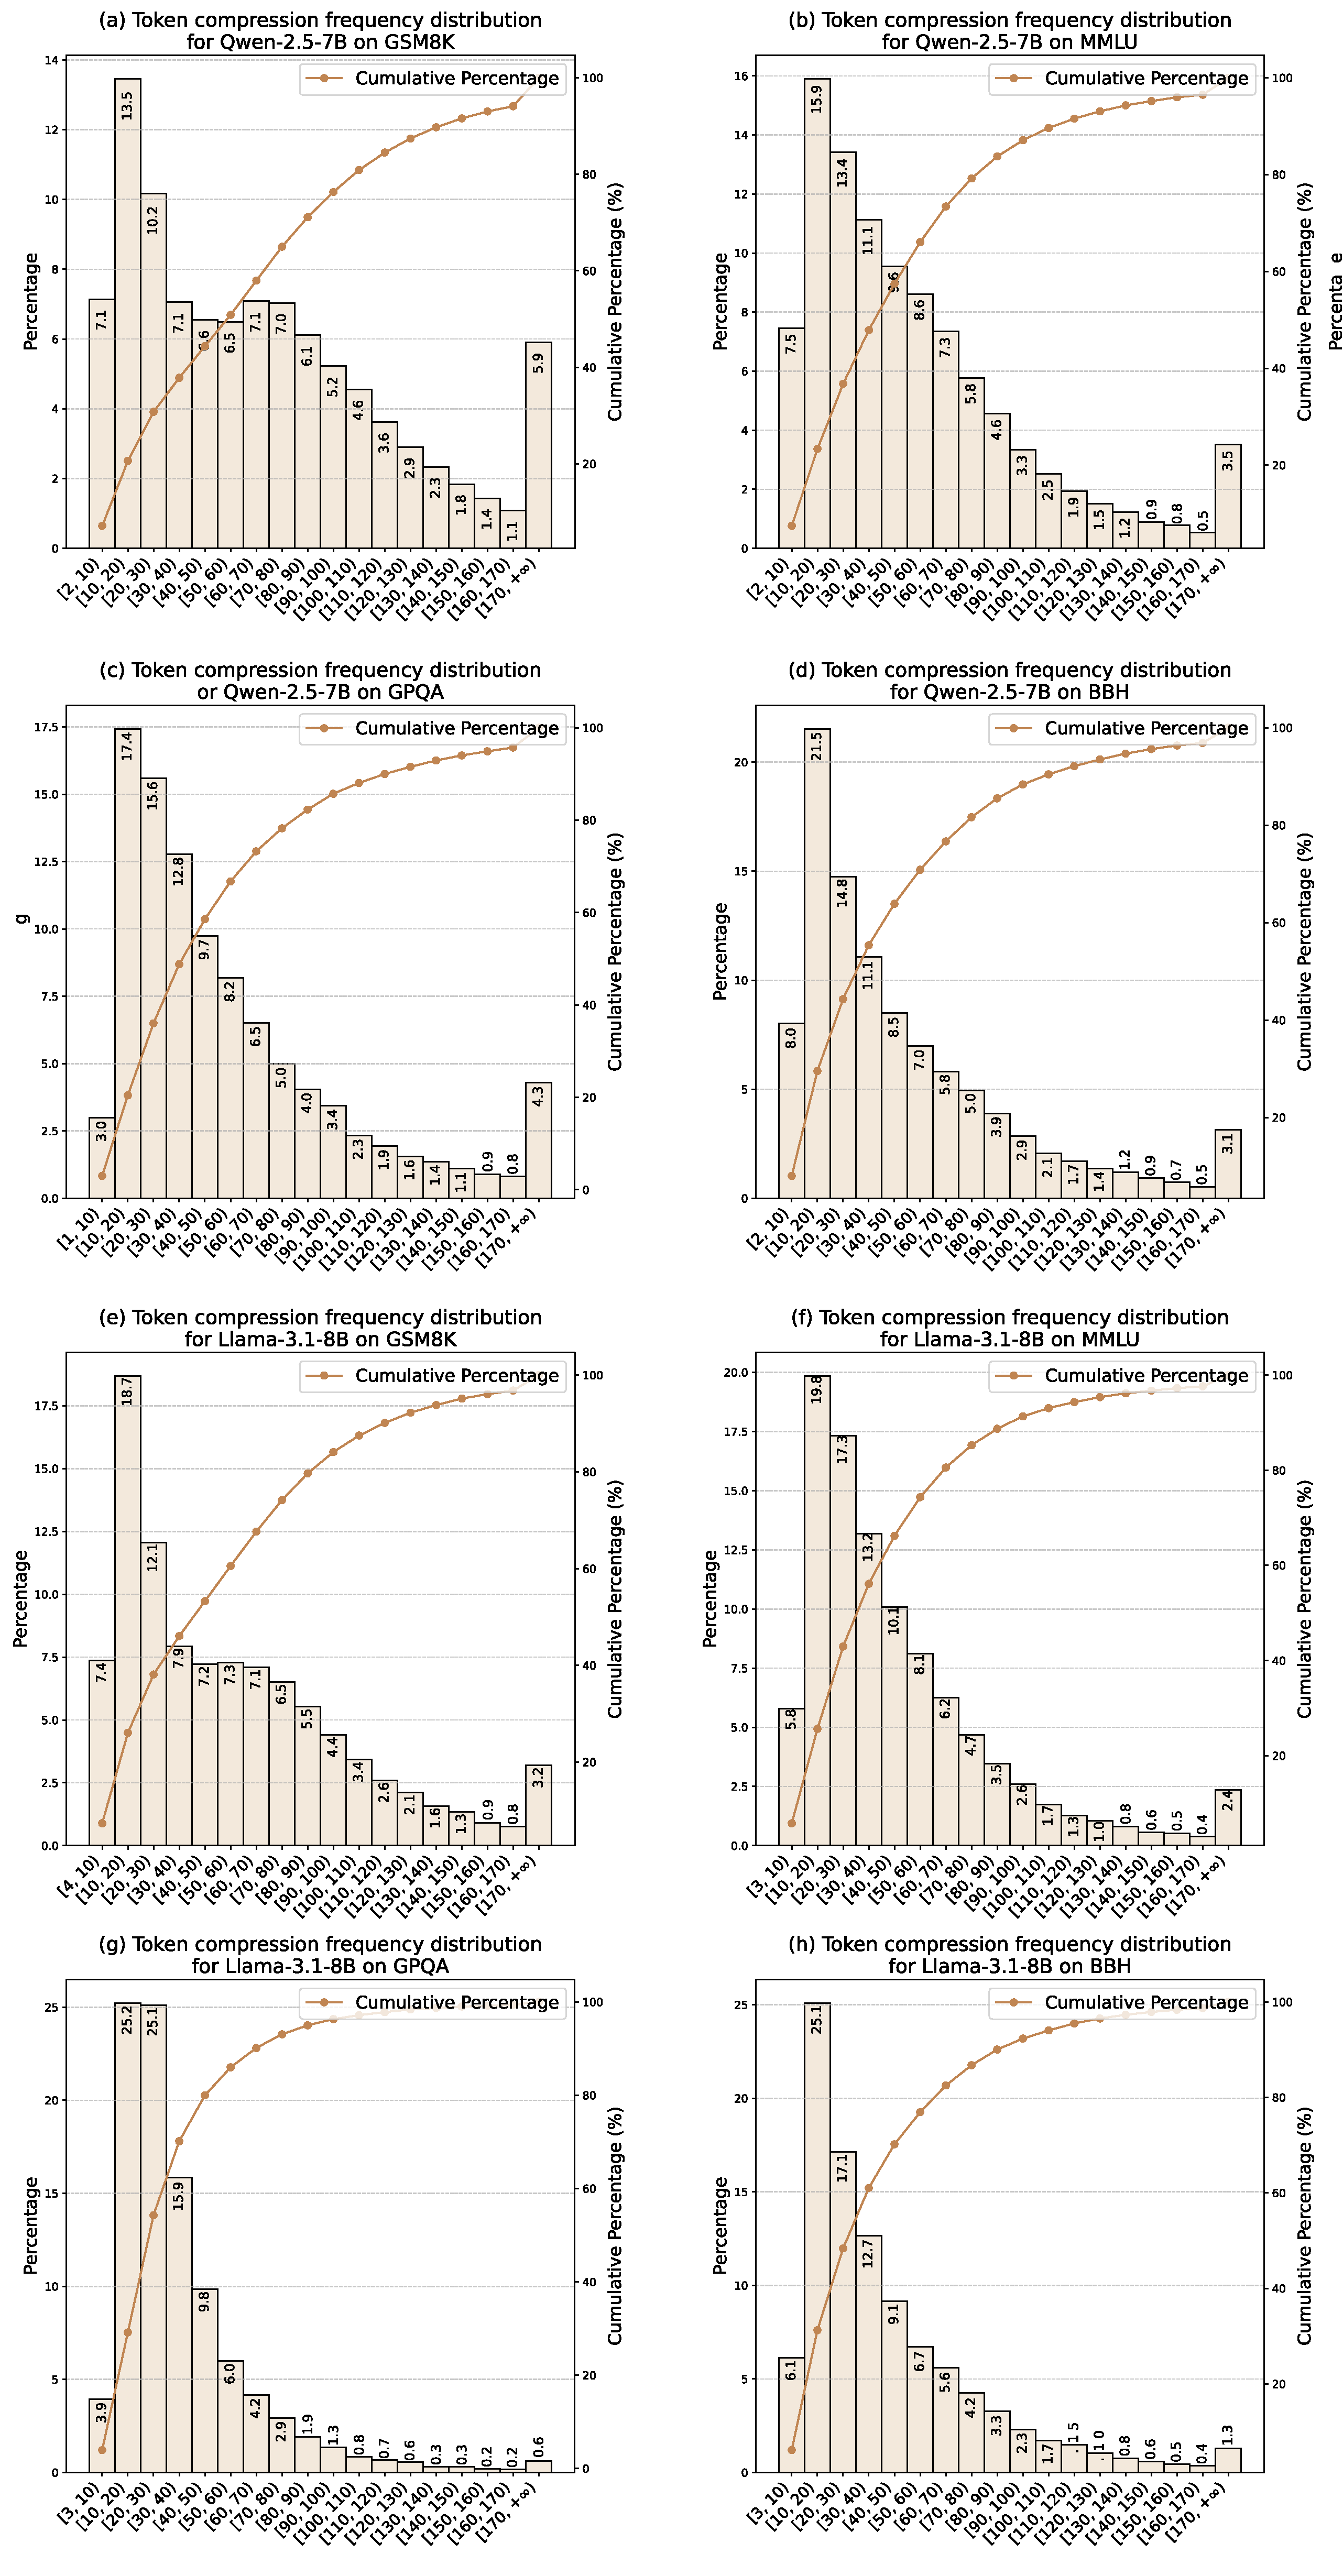
\includegraphics[width=0.76\linewidth]{figures/frequency_split.pdf} 
    }
    % \vspace{-1mm}
    \caption{Token compression frequency distribution for \ours.}
    \label{fig:app:frequency}
    % \vspace{-3mm}
\end{figure*} 


\begin{figure*}[!htbp]
\centering
\scalebox{1}{
\begin{tcolorbox}
\textbf{System Prompt:}

Below is a question. Please think through it step by step, and then provide the final answer. If options are provided, please select the correct one. 

\#\# Output format:\\
Use ``<THOUGHT>...</THOUGHT>'' to outline your reasoning process, and enclose the final answer in `\textbackslash boxed\{\}`.\\
\\
\#\# Example 1:\\
Question: \\
What is 2 + 3?\\
Output:\\
<THOUGHT>First, I recognize that this is a simple addition problem. Adding 2 and 3 together gives 5.</THOUGHT>\\
Therefore, the final answer is \textbackslash boxed\{5\}.\\
\\
\#\# Example 2:\\
Question: \\
What is 2 + 3?\\
A. 4\\
B. 5\\
C. 10\\
\\
Output:\\
<THOUGHT>First, I recognize that this is a simple addition problem. Adding 2 and 3 together gives 5.</THOUGHT>\\
Therefore, the final answer is \textbackslash boxed\{B\}.\\

\end{tcolorbox}
}

\caption{System prompt for \texttt{Qwen2.5-7B-Instruct} and \texttt{Llama3.1-8B-Instruct}.}
\label{prompt:system:base}
\end{figure*}

\begin{figure*}[!htbp]
\centering
\scalebox{1}{
\begin{tcolorbox}
\textbf{System Prompt:}

Your role as an assistant involves thoroughly exploring questions through a systematic long thinking process before providing the final precise and accurate solutions. This requires engaging in a comprehensive cycle of analysis, summarizing, exploration, reassessment, reflection, backtracing, and iteration to develop well-considered thinking process. Please structure your response into two main sections: Thought and Solution. In the Thought section, detail your reasoning process using the specified format: \texttt{<|begin\_of\_thought|>} \{thought with steps separated with `\textbackslash n\textbackslash n'\} \texttt{<|end\_of\_thought|>} Each step should include detailed considerations such as analisying questions, summarizing relevant findings, brainstorming new ideas, verifying the accuracy of the current steps, refining any errors, and revisiting previous steps. In the Solution section, based on various attempts, explorations, and reflections from the Thought section, systematically present the final solution that you deem correct. The solution should remain a logical, accurate, concise expression style and detail necessary step needed to reach the conclusion, formatted as follows: \texttt{<|begin\_of\_solution|>}  \{final formatted, precise, and clear solution\} \texttt{<|end\_of\_thought|>}  Now, try to solve the following question through the above guidelines:

\end{tcolorbox}
}

\caption{System prompt for \texttt{Vanilla}, \texttt{H2O}, \texttt{SepLLM}, \texttt{AnLLM}, and \texttt{\ours} for both Qwen-based model and Llama-based model.}
\label{prompt:system:vanilla}
\end{figure*}

\begin{figure*}[!htbp]
\centering
\scalebox{1}{
\begin{tcolorbox}
\textbf{GSM8K/MMLU/GPQA/BBH:}

Return your final response within \textbackslash boxed\{\}. \textcolor{violet}{\texttt{\{Question\}}}

\end{tcolorbox}
}

\caption{Task prompt for \texttt{Distill-R1}, \texttt{Vanilla}, \texttt{H2O}, \texttt{SepLLM}, \texttt{AnLLM}, and \texttt{\ours} for both Qwen-based model and Llama-based model.}
\label{prompt:task:r1}
\end{figure*}

\begin{figure*}[!htbp]
\centering
\scalebox{1}{
\begin{tcolorbox}
\textbf{GSM8K:}

Return your final response within \textbackslash boxed\{\}. \textcolor{violet}{\texttt{\{Question\}}}\\
\\
\textbf{MMLU:}

Please select the option that best answers the question. Return your final response within \textbackslash boxed\{\}. Here are the Question:\\
\textcolor{violet}{\texttt{\{Question\}}}\\

\textbf{GPQA:}

Given a question, please select the option that best answers it. Return your final response within \textbackslash boxed\{\}.
\textcolor{violet}{\texttt{\{Question\}}}\\


\textbf{BBH:}

Return your final response within \textbackslash boxed\{\}. If options are provided, please select the correct one. \textcolor{violet}{\texttt{\{Question\}}}

\end{tcolorbox}
}

\caption{Task prompt for \texttt{Qwen2.5-7B-Instruct} and \texttt{Llama3.1-8B-Instruct}.}
\label{prompt:task:base}
\end{figure*}

\begin{figure*}[!htbp]
\centering
\scalebox{1}{
\begin{tcolorbox}
\textbf{System Prompt:}

See Figure~\ref{prompt:system:vanilla}
\\

\textbf{Input:}

Return your final response within \textbackslash boxed\{\}. The average of the numbers 23 and $x$ is 27. What is the positive difference between 23 and $x$? (Recall that the average of two numbers is their sum divided by 2).
\\

\textbf{Output:}

\texttt{<|begin\_of\_thought|>}
Okay, let's see. The problem says that the average of the numbers 23 and x is 27. We need to find the positive difference between 23 and x. Hmm, right. Since the average of two numbers is their sum divided by 2, I can start by setting up the equation for the average.\textcolor{red}{\texttt{<w>}}So, the average of 23 and x is (23 + x)/2. According to the problem, this average equals 27. So I can write the equation:\textcolor{red}{\texttt{<w>}}(23 + x)/2 = 27\textcolor{red}{\texttt{<w>}}To find x, I should solve this equation. Let me multiply both sides by 2 to get rid of the denominator. That gives:\textcolor{red}{\texttt{<w>}}23 + x = 54\textcolor{red}{\texttt{<w>}}Then, subtract 23 from both sides to isolate x:\textcolor{red}{\texttt{<w>}}x = 54 - 23\textcolor{red}{\texttt{<w>}}Calculating that, 54 minus 23 is 31. So x is 31. Now, the question asks for the positive difference between 23 and x. The positive difference would be the absolute value of 23 - x. Since x is 31, that's |23 - 31|, which is | -8 |, so 8. Alternatively, it could also be |31 - 23|, which is the same result, 8. Either way, the positive difference is 8.\textcolor{red}{\texttt{<w>}}Wait, let me check my steps again to make sure I didn't make a mistake. Starting with the average: (23 + x)/2 = 27. Multiply both sides by 2: 23 + x = 54. Subtract 23: x = 31. Difference between 23 and 31 is 8. That seems right. Yeah, I think that's correct. No issues here.\textcolor{red}{\texttt{<w>}}
\texttt{<|end\_of\_thought|>}

\texttt{<|begin\_of\_solution|>}
\textcolor{red}{\texttt{<w>}}The average of 23 and \( x \) is given by \(\frac{23 + x}{2} = 27\). Multiplying both sides by 2:  
\[
23 + x = 54
\]  
Subtracting 23 from both sides:  
\[
x = 54 - 23 = 31
\]  
The positive difference between 23 and \( x \) is:  
\[
|31 - 23| = 8
\]  \textcolor{red}{\texttt{<w>}}\(\boxed{8}\)
\texttt{<|end\_of\_solution|>}

\end{tcolorbox}
}

\caption{A training case. \texttt{<w>} is a compression trigger.}
\label{prompt:case:train}
\end{figure*}
% 这边需要高亮一下
\begin{figure*}[!t]
\centering
\scalebox{0.9}{
\begin{tcolorbox}
\textbf{Question:}\\
Boris owns a chocolate factory. He produces 50,000 bars of chocolate each month. Boris produces 8,000 bars of chocolate the first week. The second week, Boris only produces half as much as the first week. But, the third week, Boris produces three times as much as the first week. How much does he produce the fourth week?\\ \\
\textbf{Model Output:}\\
\texttt{<|begin\_of\_thought|>} \\
Okay, let's see. Boris has a chocolate factory that produces 50,000 bars each month. The question is asking how much he produces in the fourth week. Hmm, let me break this down step by step.
<|splitter|>\\ 
\\First, the total monthly production is 50,000 bars. The month is divided into four weeks, right? So the production for each week adds up to 50,000. The problem gives the production for the first three weeks and asks for the fourth week. Let me note down the given information.
<|splitter|>\\
\\First week: 8,000 bars. That's straightforward. Then the second week, he produces half as much as the first week. Half of 8,000 is 4,000. So second week is 4,000 bars. Then the third week, he produces three times as much as the first week. Three times 8,000 is 24,000. So third week is 24,000 bars.
<|splitter|>\\
\\Now, to find the fourth week's production, I need to subtract the sum of the first three weeks from the total monthly production. Let me add up the first three weeks: 8,000 + 4,000 + 24,000. Let's do the math step by step. 8,000 plus 4,000 is 12,000. Then 12,000 plus 24,000 is 36,000. So the total for the first three weeks is 36,000 bars.
<|splitter|>\\
\\The total monthly production is 50,000 bars. Subtracting the first three weeks from the total gives the fourth week's production. So 50,000 minus 36,000 equals 14,000 bars. Therefore, Boris produces 14,000 bars in the fourth week.
<|splitter|>\\ 
\\Wait a second, let me double-check my calculations to make sure I didn't make a mistake. First week: 8,000. Second week: half of 8,000 is indeed 4,000. Third week: three times 8,000 is 24,000. Adding those: 8,000 + 4,000 = 12,000; 12,000 + 24,000 = 36,000. Total monthly is 50,000. So 50,000 - 36,000 = 14,000. Yep, that seems right. I don't think I missed anything here. The problem states the production for each week as fractions or multiples of the first week, so the calculations are straightforward. No complicated formulas needed. Just basic arithmetic. So the answer should be 14,000 bars in the fourth week.
<|splitter|>\\
\texttt{<|end\_of\_thought|>}\\
\\ \texttt{<|begin\_of\_solution|>}
\\Boris's weekly chocolate production is calculated as follows:
<|splitter|>\\
\\- \textbf{First week}: 8,000 bars  \\
- \textbf{Second week}: \( \frac{8,000}{2} = 4,000 \) bars \\ 
- \textbf{Third week}: \( 8,000 \times 3 = 24,000 \) bars  <|splitter|>\\
\\Total for the first three weeks:  \\
$4,000 + 4,000 + 24,000 = 32,000 \text{ bars}$
<|splitter|> \\
\\Subtracting this from the monthly total: \\ 
$50,000 - 32,000 = 18,000 \text{ bars}$
<|splitter|>\\
\\Thus, Boris produces \(\boxed{18000}\) bars in the fourth week. <|splitter|>\\
\texttt{<|begin\_of\_solution|>}

\end{tcolorbox}
}

\caption{Bad Case. \texttt{<|splitter|>} is equal to \texttt{<w>} in Figure~\ref{prompt:case:train}.}
\label{prompt:case}
\end{figure*}

\subsection{Why \ours~generates more tokens with smaller cache size?}
As shown in Figure~\ref{fig:exp:efficient}(e-f), we find that \ours~generates more tokens with smaller cache size.
We examined outputs under different cache sizes and found that when the cache size is small, the model tends to repeat previous content more often. 
We believe this is because smaller cache sizes lead to greater information loss during compression, prompting the model to regenerate earlier content more frequently to retain as much information as possible.

\subsection{Comparison with Implicit CoT Works}
\begin{table*}[h!]
\small
\centering
\begin{tabular}{lcccc}
\toprule
\textbf{Method} & \textbf{Memory Optimization} & \textbf{Training Cost} & \textbf{Interpretability} & \textbf{Generalization} \\
\midrule
System-1.5~\cite{arxiv25_system_1_5} & Significant & High  & Weak & Weak \\
SoftThinking~\cite{arxiv25_soft_thinking}  & Limited    & None  & Weak & Good \\
\ours & Significant & Low   & Good & Good \\
\bottomrule
\end{tabular}
\caption{Comparison of different methods.}
\label{tab:app:comparison}
\end{table*}

Both our work and implicit CoT methods operate in continuous spaces.
While implicit CoT performs reasoning entirely in continuous space, \ours~employs a hybrid approach combining continuous and discrete space reasoning. 
The overview differences are shown in Table~\ref{tab:app:comparison}.
Below we clarify the key differences:
\begin{itemize}
    \item \textbf{Reasoning Acceleration Mechanism}.
    \emph{Implicit CoT} methods (e.g., System-1.5~\cite{arxiv25_system_1_5}, SoftThinking~\cite{arxiv25_soft_thinking}) accelerate reasoning by reducing generation steps through continuous token representations. 
    The entire reasoning process depends on full context.
    \emph{\ours} accelerates inference by reducing the number of historical tokens needed for generation, without requiring full context dependence.

    \item \textbf{Training Approach.}
    Implicit CoT typically requires complex, multi-stage training with significant overhead (e.g., System-1.5's two-phase training~\cite{arxiv25_system_1_5} or Coconut's curriculum learning~\citep{arxiv24_coconut}). Some methods~\cite{arxiv25_soft_thinking, arxiv24_ccot} even require architecture modifications.
    \ours~uses standard SFT with modified attention masks, requiring neither specialized training data nor architectural changes.

    \item \textbf{Interpretability and Generalization}.
    Current implicit CoT methods face interpretability challenges (due to continuous reasoning) and limited out-of-domain generalization (except SoftThinking~\cite{arxiv25_soft_thinking}).
    \ours~maintains discrete tokens for better interpretability and shows promising out-of-domain generalization in our experiments, as shown in Table~\ref{tab:app:comparison}.

\end{itemize}

% \section{Future Work}
